% !TEX root = ParticleFilter.tex
\section{Method\label{method}}


\subsection{The Agent-Based Model: StationSim}

\textit{StationSim} is a simple agent-based model that has been designed to very loosely represent the behaviour of a crowd of people moving from an entrance on one side of a rectangular environment to an exit on the other side. This is analogous to a train arriving at a train station and passengers moving across the concourse to leave. A number of agents, $N$, which varies in the later experiments, are created when the model starts. They are able to enter the environment (leave their train) at a uniform rate through one of three entrances. They move across the `concourse' and then leave by one of the two exits. The entrances and exits have a set size, such that only a limited number of agents can pass through them in any given iteration. Once all agents have entered the environment and passed through the concourse then the simulation ends. The model environment is illustrated in Figure \ref{fig:StationSim}, with the trajectories of two interacting agents for illustration. 
%The model is also outlined in full as per the ODD protocol~\citep{grimm_odd_2010} in Appendix~\ref{odd}.

\begin{figure}[ht]
\centering
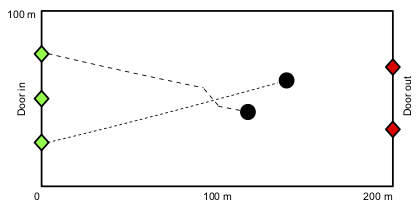
\includegraphics[width=0.5\textwidth]{figures/PF_ABM}
\caption{StationSim environment with 3 entrance and 2 exit doors}.\label{fig:StationSim}
\end{figure}

The model has deliberately been designed to be extremely simple and does not attempt to match the behavioural realism offered by more developed crowd models \citep{chen_multiagentbased_2017, helbing_simulating_2000, klugl_largescale_2007, vanderwal_simulating_2017}. The reason for this simplicity is so that: (1) the model can execute relatively quickly; (2) the probabilistic elements in the model are limited (we know precisely from where probabilistic behaviour arises); (3) the model can be described fully using a relatively simple state vector, as discussed in Section~\ref{state_vector}. Importantly, the model is able to capture the emergence of \textit{crowding}. This results because each agent has a different maximum speed that they can travel at. Therefore, when a fast agent approaches a slower one, they attempt to get past by making a random binary choice to move left or right around them. Depending on the agents in the vicinity, this behaviour can start to lead to the formation of crowds. To illustrate this, Figure~\ref{fig:crowding} shows the paths of the agents (\ref{fig:crowding-trails}) and the total agent density (\ref{fig:crowding-density}) during an example simulation.   The degree and location of crowding depends on the random allocation of maximum speeds to agents and their random of direction taken to avoid slower agents; these cannot be estimated \textit{a priori}. Unlike in previous work where the models did not necessarily meet the common criteria that define agent-based models \citep[e.g.]{lloyd_exploring_2016, ward_dynamic_2016} this model respects three of the most important characteristics: 

\begin{figure}
    \centering
    \begin{subfigure}[b]{0.48\textwidth}
        \centering
        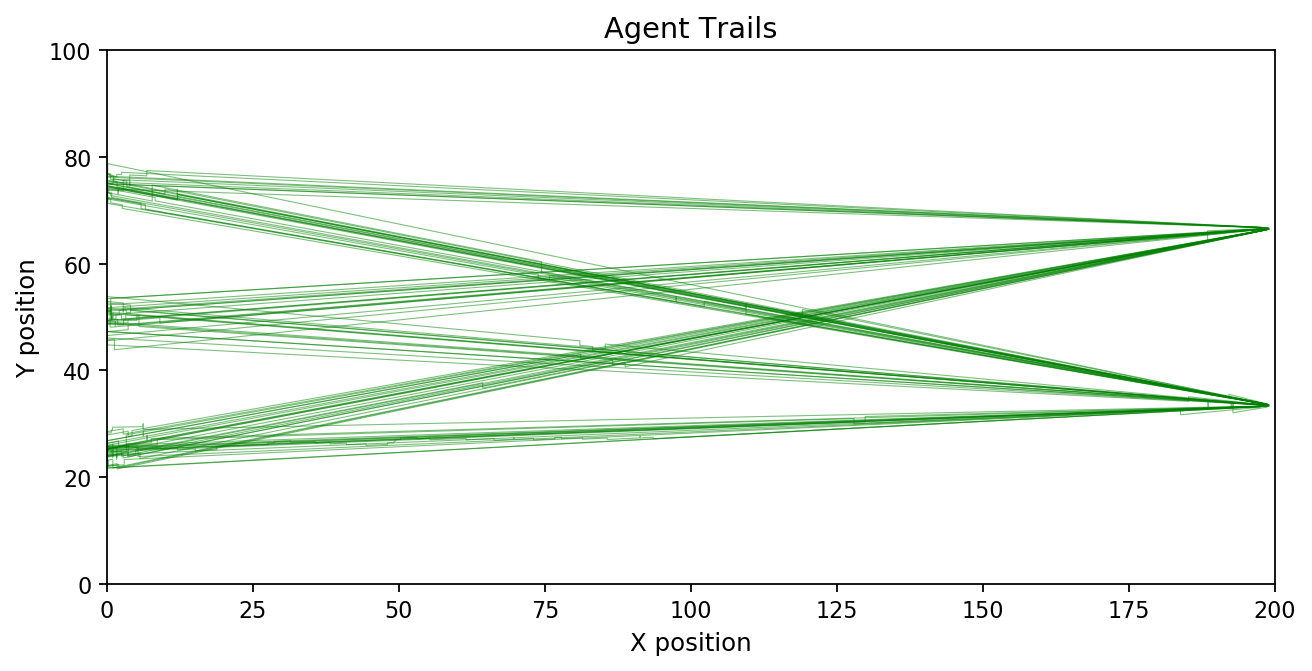
\includegraphics[width=.95\linewidth]{figures/crowding-trails}
        \caption{Individual trails showing the paths taken by agents}
        \label{fig:crowding-trails}
    \end{subfigure}
    \label{fig:crowding}
    \begin{subfigure}[b]{0.48\textwidth}
        \centering
        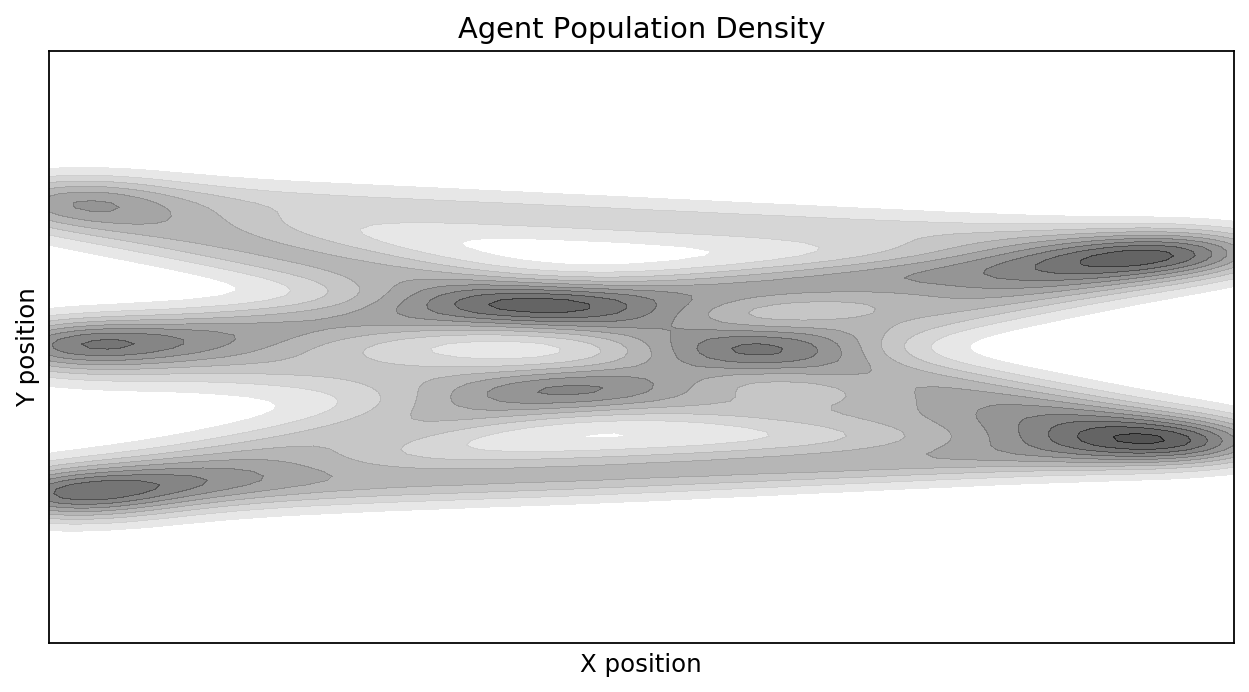
\includegraphics[width=.95\linewidth]{figures/crowding-density}
        \caption{The total crowd density over the simulation run.}
        \label{fig:crowding-density}
    \end{subfigure}
    \caption{An example of crowding in the StationSim model}
    \label{fig:crowding}
\end{figure}

\begin{itemize}
	\item individual heterogeneity -- agents have different maximum travel speeds; 
	\item agent interactions -- agents are not allowed to occupy the same space and try to move around slower agents who are blocking their path; 
	\item emergence -- crowding is an emergent property of the system that arises as a result of the choice of exit that each agent is heading to and their maximum speed.
\end{itemize}

The model code is relatively short and easy to understand. It is written in Python, and is available in its entirety at in the project repository \citep{stationsimgit}.
% \footnote{\url{XXXX Link to repo}}.


\subsection{Data Assimilation - Introduction and Definitions}

DA methods are built on the following assumptions: 

\begin{enumerate}
	\item Although they have low uncertainty, observational data are often spatio-temporally sparse. Therefore there are typically insufficient amounts of data to to describe the system in sufficient detail and a data-driven approach would not work.
	\item Models are not sparse; they can represent the target system in great detail and hence fill in the spatio-temporal gaps in observational data by propagating data from observed to unobserved areas \citep{carrassi_data_2018}. For example, some parts of a building might be more heavily observed than others, so a model that assimilated data from the observed areas might be able to estimate the state of the unobserved areas. However, if the underlying systems are complex, a model will rapidly diverge from the real system in the absence of \textit{up to date} data \citep{ward_dynamic_2016}.
	\item The combination a model and up-to-date observational data allow ``all the available information'' to be used to determine the state of the system as accurately as possible \citep{talagrand_use_1991}. 
\end{enumerate}

DA algorithms work by running a model forward in time up to the point that some new observational data become available. This is typically called the \textit{predict} step. At this point, the algorithm has an estimate of the current system state and its uncertainty (the prior). The next step, \textit{update},  involves using the new observations, and their uncertainties, to update the current state estimate to create a posterior estimate of the state. As the posterior has combined the best guess of the state from the model \textit{and} the best guess of the state from the observations, it should be a closer estimate of the true system state than that which could be estimated from the observations or the model in isolation.

\subsection{The Particle Filter\label{particle_filter}}

There are many different ways to perform data assimilation, as discussed in Section \ref{da_pf}. Here, a potentially appropriate solution to the data assimilation problem for agent-based models is the particle filter -- also known as a Bayesian bootstrap filter or a sequential Monte Carlo method -- which represents the posterior state using a collection of model samples, called particles \citep{gordon_novel_1993,carpenter_improved_1999,wang_data_2015, carrassi_data_2018}. Figure~\ref{fig:PF_flowchart} illustrates the process of running a particle filter. Note that the `pseudo-truth model' is a single instance of the agent-based model that is used as a proxy for the real system as per the identical twin experimental framework that we have adopted.

The data assimilation `window' determines how often new observations are assimilated into the particle filter. The size of the window is an important factor -- larger windows result in the particles deviating further from the real system state -- but here we fix the window at 100 iterations. The simulation terminates when all agents have left the system.

\begin{figure}[ht]
\centering
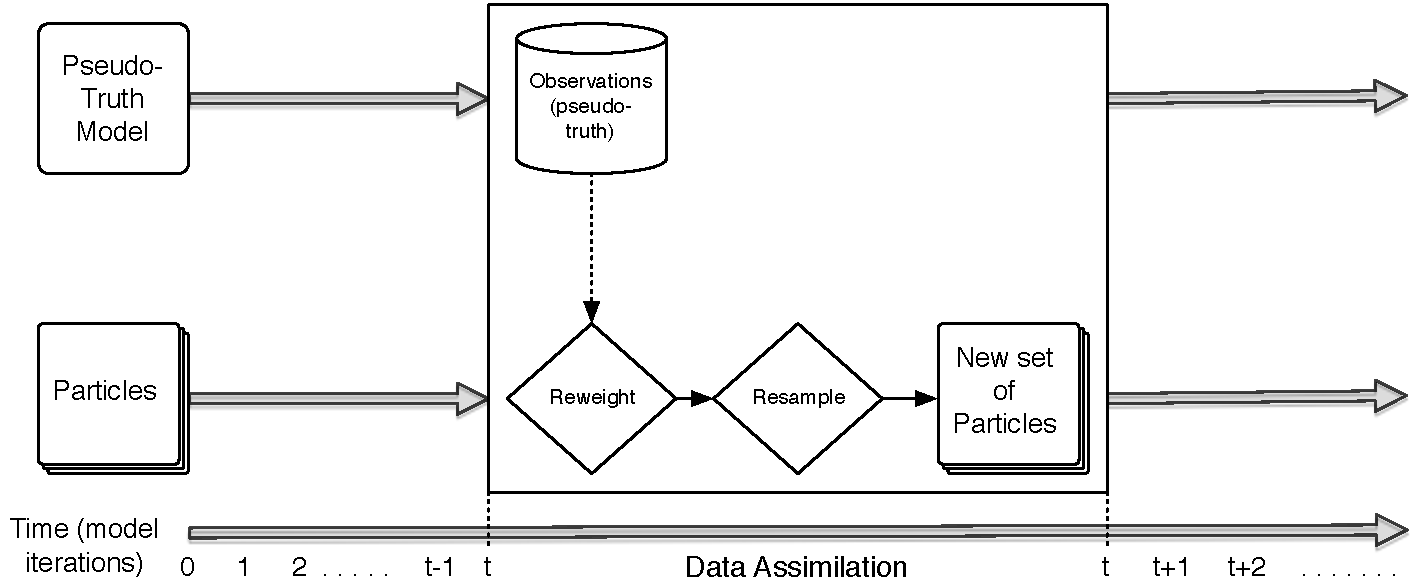
\includegraphics[width=0.8\textwidth]{figures/PF_flowchart2}
\caption{Flowchart of data assimilation process using a particle filter.\label{fig:PF_flowchart}}
\end{figure}

\subsubsection{The State Vector and Transition Function\label{state_vector}} 

Here, the \textit{state vector}, at a time $t$, contains all the information that a transition function needs to iterate the model forward by one step, including all of the agent ($i = \{ 0, 1, \dots, N \} $) parameters ($\overrightarrow{p_i}$) and variables ($\overrightarrow{v_i}$) as well as global model parameters $\overrightarrow{P}$:
\begin{equation}
  S_t  = \left[ \begin{array}{cccccccc}
\overrightarrow{p_0} & \overrightarrow{v_0} & \overrightarrow{p_1} &  \overrightarrow{v_1} &  \dots &  \overrightarrow{p_N} &  \overrightarrow{v_N} & \overrightarrow{P} 
\end{array} \right]
\end{equation} 

A similar structure, the \textit{observation vector}, contains all of the observations made from the `real world' (in this case the pseudo-truth model) at a time $t$. Here, the particle filter is only used to estimate the state of the models variables ($\overrightarrow{v_i}$), not any of the parameters ($\overrightarrow{p_i}$ and $\overrightarrow{P}$) (although it is worth noting that parameter estimation is technically feasible and will be experimented with in future work). Also, the current speed of an agent can be calculated from its current location and the locations of the agents surrounding it, so in effect the observation vector only needs to include the positions of the agents with the addition of some Gaussian noise, $\epsilon$:
\begin{equation}
  O_t  = \left[ \begin{array}{ccccccc}
x_0 & y_0 & x_1 & y_1 & \dots & x_n & y_n 
\end{array} \right]
\end{equation} 

 Therefore in the experiments conducted here, all model parameters are fixed. Hence a further vector is required to map the observations to the state vector that the particles can actually manipulate. We define the partial state vector $S'$ to match the shape of $O$, i.e.:
\begin{equation}
  S'_t  = \left[ \begin{array}{ccccccc}
x_0 & y_0 & x_1 & y_1 & \dots & x_n & y_n 
\end{array} \right]
\end{equation} 

This has the effect of `pairing' agents in the particles to those in the pseudo-truth data, in a similar approach to that taken by \citep{wang_data_2015}. It is worth noting that, because the particle filter will not be tasked with parameter estimation, then the data assimilation is somewhat simpler than it would be in a real application. For example, one of the agent parameters is used to store the location of the exit out of the environment that the agent is moving towards. As this parameter is set \textit{a priori} for each agent, then the particle filter does not need to estimate where the agents are ultimately going, only where they currently are.

\subsubsection{Observations from the pseudo-truth data}

In a real application, the particle filter would be assimilating data in real time from sensors of the real world. This is not the case here so instead, we take `observations' from the pseudo-truth data (which are, as it happens, generated by the StationSim model). Each particle evolves in time according to the StationSim dynamics and receives new observations at regular intervals. Measurement error (i.e. noise, $\epsilon$) is added to the observations (in the real world, sensors observations will be noisy). Here, observations take the form of the $(x,y)$ locations of all agents. This is analogous to tracking all individuals in a crowd and providing snapshots of their locations at discrete points in time to the particle filter. This `synthetic observation' is probably more detailed than reality, so future work will vary the amount of detail provided to the algorithm. It will firstly reduce the number of agents who are observed (e.g. tracking only \textit{some} people) and then provide only aggregate population counts (which is analogous to using a camera or other sensor to count the number of people at a certain point). 

\subsubsection{Particle Weights}

Each particle in the particle filter has a weight associated with it that quantifies how similar a particle is to an observation. The weights are calculated at the end of each data assimilation window (i.e. when observations become available). At the start of the following window the particles then evolve independently from each other \citep{fearnhead_particle_2018}.  The weights are, in effect, the average distance between agents in that particle and the corresponding agents in StationSim (recall that there is a one-to-one mapping between agents in the particles and agents in the truth model). Formally, let $x^n(i,t)$ be the location of the $i$-th agent at time $t$ in the $n$-th particle for $n \in \{1,\dots,N\}$ and let $x(i,t)$ be the location of the $i$-th agent in StationSim for $i \in \{1,\dots,I\}$. The error of the $n$-th particle $\epsilon^n(t)$ at time $t$ is then given by
\begin{equation}
\epsilon^n(t) = \frac{1}{I} \sum_{i=1}^I |x(i,t) - x^n(i,t)|,
\end{equation}
and the particle filter error $\nu(t)$ at time $t$ is given by
\begin{equation}
\label{eqn:particle_error}
\begin{split}
\nu(t) =& \frac{1}{N} \sum_{n=1}^{N} \epsilon^n(t), \\
=& \frac{1}{NI} \sum_{n=1}^{N}\sum_{i=1}^I |x(i,t) - x^n(i,t)|.
\end{split}
\end{equation}

It is worth noting that, because the agent locations are the only data stored in the partial state vector, the particle error is equivalent to the Euclidean distance ($l_2$-norm) between the particle partial state vector $S'_{t}$ and the observation vector $O_t$,
\begin{equation}
 \nu(t) = || S'_{t} - O_t  ||_2.
\end{equation} 

Particles with relatively large error are likely to be removed during the sampling procedure (discussed in the following section), whereas those with low error are likely to be duplicated. In addition for their use in resampling, the population of particle weights can be used to gain insight into how well the particle filter is able to represent the `true' system state overall. 

\subsubsection{Sampling Procedure\label{particle_sampling}}

Here, a bootstrap filter is implemented which uses systematic resampling \citep{doucet_introduction_2001, douc_comparison_2005, wang_data_2015, long_spatial_2017, carrassi_data_2018}. This begins by taking a random sample $U$ from the uniform distribution on the interval $[0,1/N]$ and then selecting $N$ points $U^i$ for $i \in \{1,\dots,N\}$ on the interval $[0,1]$ such that
\begin{equation}
U^i = (i-1)/N + U.
\end{equation}
Let the particles currently have locations $x_i$. Using the inversion method, we calculate the cumulative sum of the normalised particle weights $w_i$ and define the inverse function $D$ of this cumulative sum, that is:
\begin{equation}
D(u) = i \text{ for } u \in \left(\sum_{j=1}^{i-1}w_j,\sum_{j=1}^{i}w_j\right].
\end{equation}
Finally, the new locations of the resampled particles are given by $x_{D(U^i)}$.

As discussed in Section~\ref{background}, a well-studied issue that particle filters face is that of particle deprivation \citep{snyder_obstacles_2008}, which refers to the problem of particles converging to a single point such that all particles, but one, vanish \citep{kong_sequential_1994}.  
% This vastly reduces the size of the state space covered by the population of particles and will make it difficult or impossible to find particles with low error in later windows. Common approaches to resolve the deprivation problem include increasing the number of particles or trying to reduce the dimensionality of the state space. Bespoke approaches also exist; for example \citep{wang_data_2015} develop a technique called `component set resampling' that samples \textit{parts} of particles (i.e. those parts that are working well) rather than whole particles in their entirety.  
Here, the problem is addressed in two ways. Firstly by simply using large numbers of particles relative to the size of the state space and, secondly, by diversifying the particles \citep{vadakkepat_improved_2006} -- also known as roughening, jittering, and diffusing \citep{li_fight_2014, shephard_learning_2009, pantrigo_combining_2005}. In each iteration of the model we add Gaussian white noise to the particles' state vector to increase their variance, which increases particle diversity. This encourages a greater variety of particles to be resampled and therefore makes the algorithm more likely to represent the state of the underlying model. This method is a special case of the resample-move method presented in \citep{gilks_following_2001}. The amount of noise to add is a key hyper-parameter -- too little and it has no effect, too much and the state of the particles moves far away from the true state -- as discussed in the following section. 
